\chapter{Estado del arte}


%=========================================================
%                                                         Estado del arte
%=========================================================
%\section{Estado del arte}
\noindent En esta sección se describen las aplicaciones web existentes más relacionadas con el tema del presente Trabajo Terminal:


%=========================================================
%                                                         Historia
%=========================================================
%\section{Historia}


%=========================================================
%                                                         Aplicaciones
%=========================================================
\section{Aplicaciones}
\noindent Dentro de la investigación que se realizo con respecto a sistemas o aplicaciones web que tuviesen el mismo objetivo al proyecto propuesto. A continuación se muestran las aplicaciones que se encontraron, así como una descripción de su funcionamiento y las principales caracteristicas de cada una de ellas.
\section{Aplicaciones Tournament Software}
\noindent Esta aplicación ofrece al usuario un plataforma en la que puede registrar equipos deportivos, a su vez le ofrece crear ligas (competencias) entre los equipos que previamente registro, agregando que al final le dará una tabla de posiciones de los equipos y si este desea ver más información de uno en particular, desglosar la información en otra vista. \cite{ts}
Características: 
\begin{itemize}
	\item Login
	\item Registro de equipos
	\item Creación de eventos
	\item Consulta de resultados
\end{itemize}
\pagebreak
%=========================================================
%                                                         Imagenes
%=========================================================
\begin{figure}[h]
	\centering
	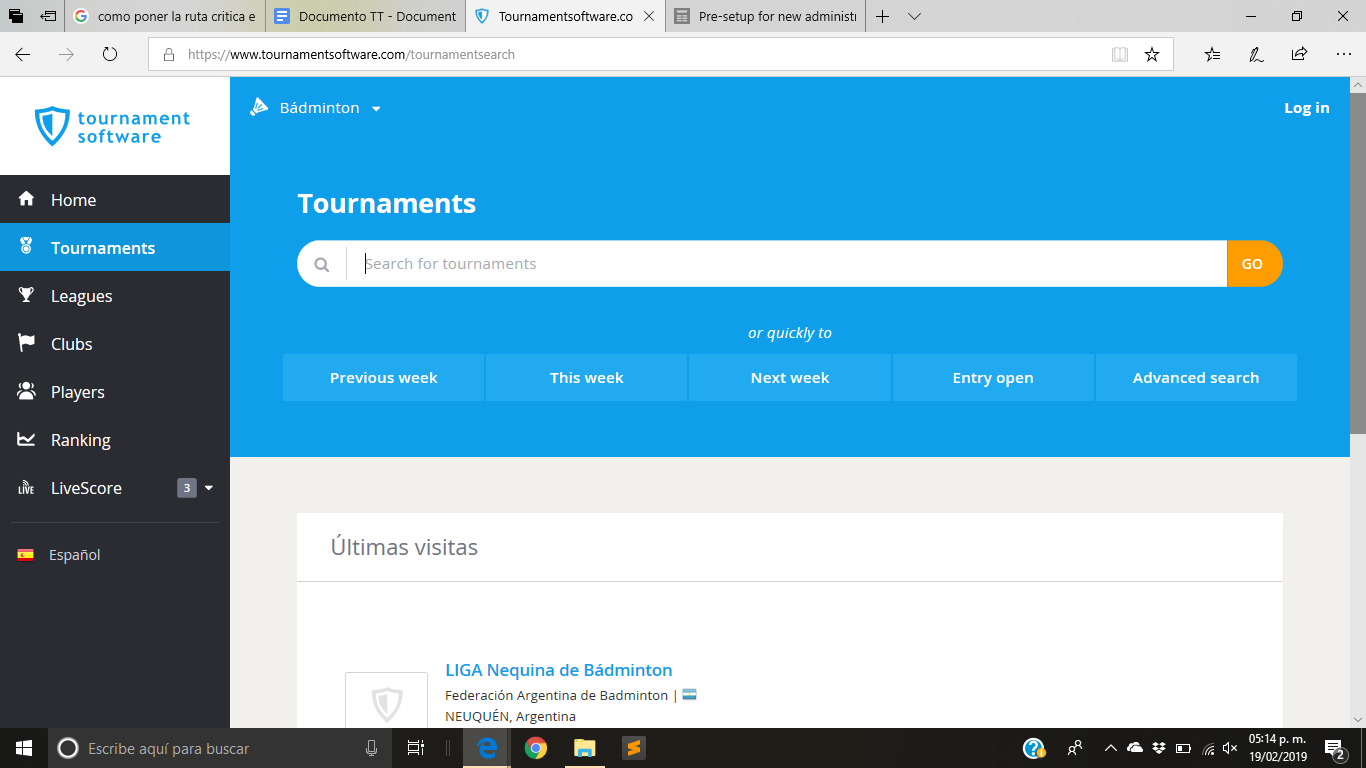
\includegraphics[width=12cm, height=6cm]{Imagenes/Aplicaciones/ToS1.png}
	\caption{Eventos registrados}
\end{figure}
\begin{figure}[h]
	\centering
	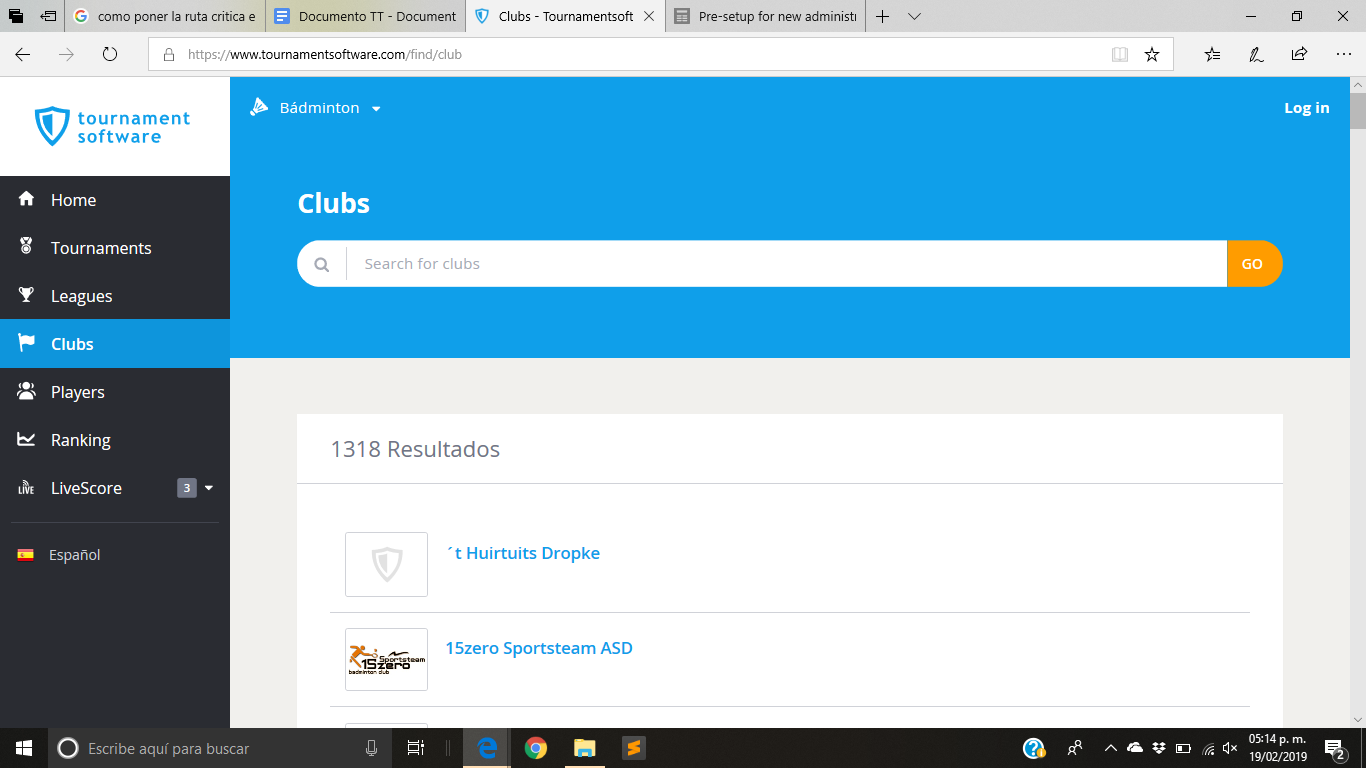
\includegraphics[width=12cm, height=6cm]{Imagenes/Aplicaciones/ToS2.png}
	\caption{Clubs registrados}
\end{figure}
\pagebreak
\begin{figure}[h]
	\centering
	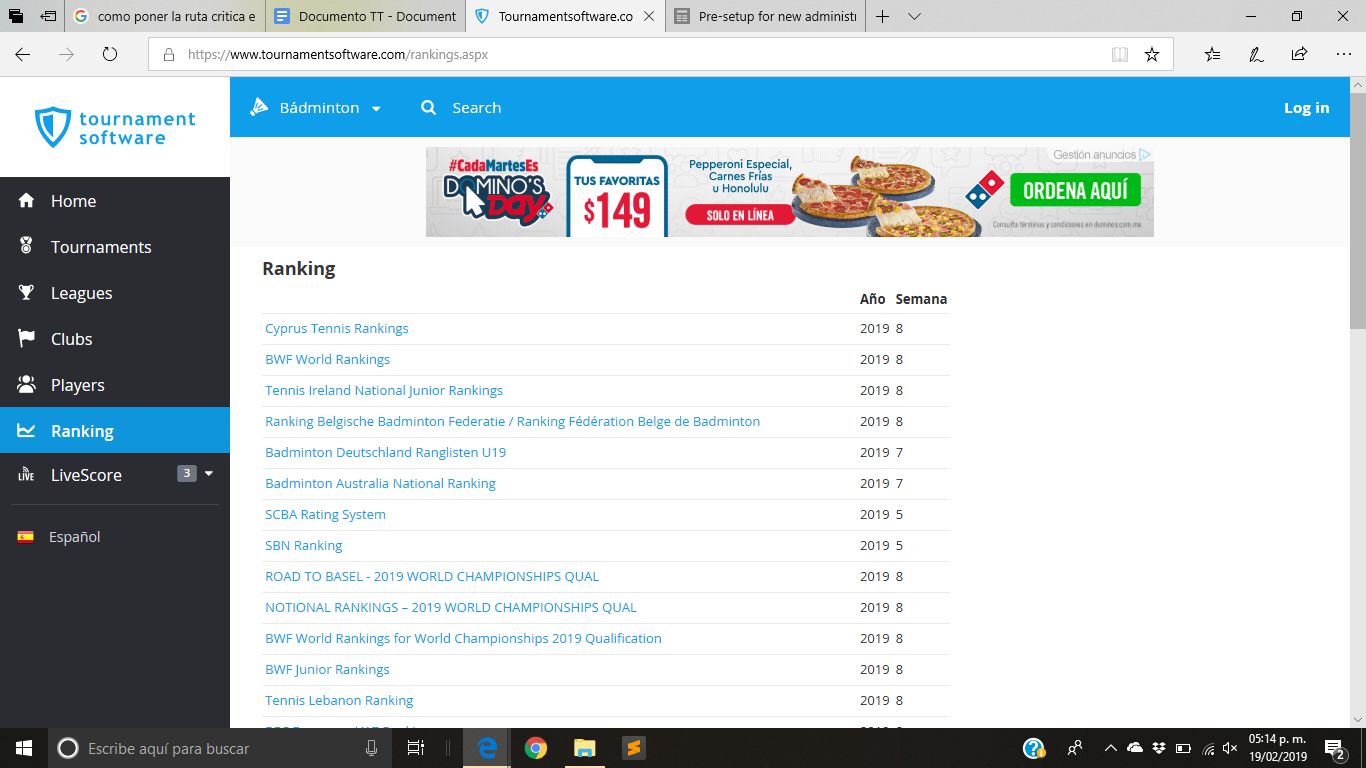
\includegraphics[width=12cm, height=6cm]{Imagenes/Aplicaciones/Tos3.png}
	\caption{Resultados}
\end{figure}

\section{Aplicaciones Active Network}
\noindent Esta aplicación ofrece a los usuarios de un manera organizada y fácil, el controlar alguna actividad deportiva, a su vez tienen un mercado más amplio ya que ofrecen sus servicio a escuelas, eventos deportivos, entre otros. Una desventaja que se encontró, es que para cada actividad deportiva se tiene una página designada, que es independiente al resto. \cite{act}
Características: 
\begin{itemize}
	\item Login
	\item Calendario
	\item Registro de equipos
	\item Reportes
	\item Registro de eventos
\end{itemize}
%=========================================================
%                                                         Imagenes
%=========================================================
\begin{figure}[ht]
	\centering
	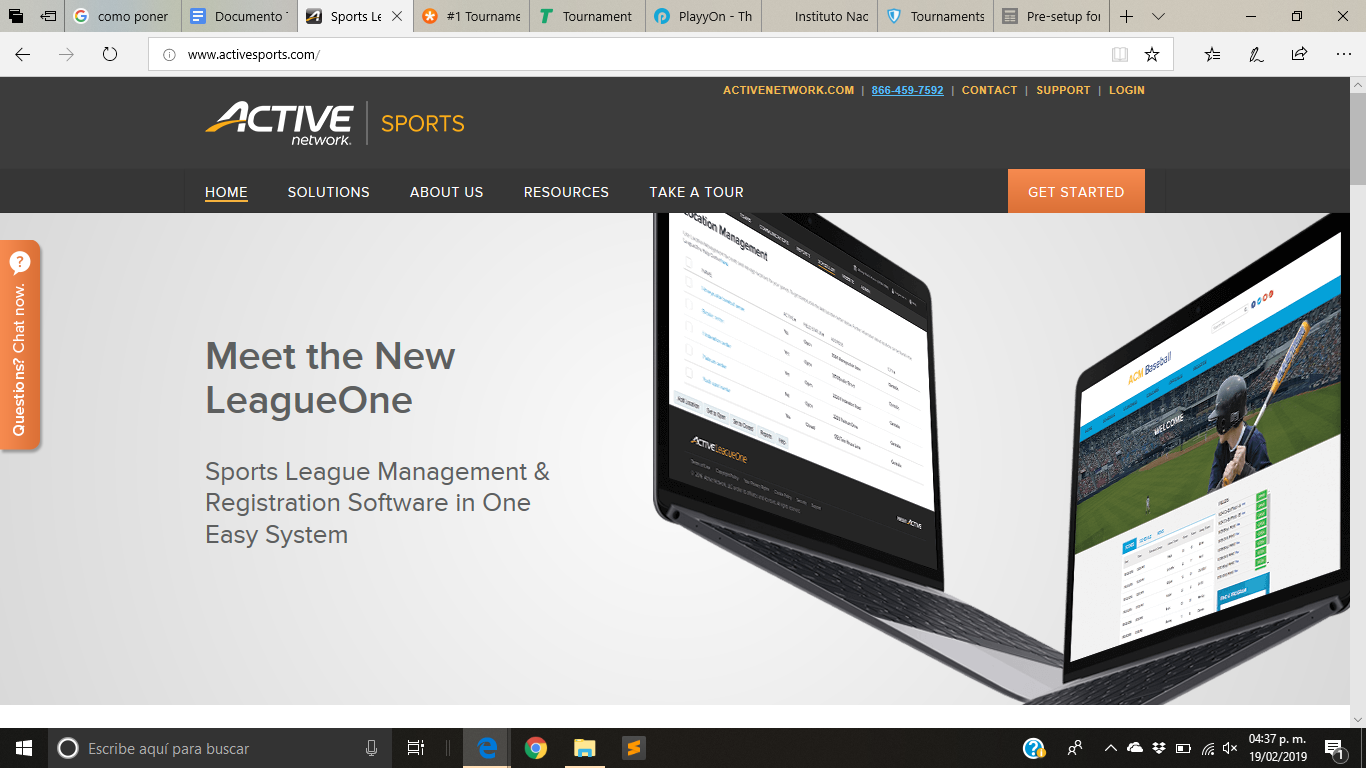
\includegraphics[width=12cm, height=6cm]{Imagenes/Aplicaciones/AN1.png}
	\caption{Página principal}
\end{figure}

\pagebreak

\begin{figure}[ht]
	\centering
	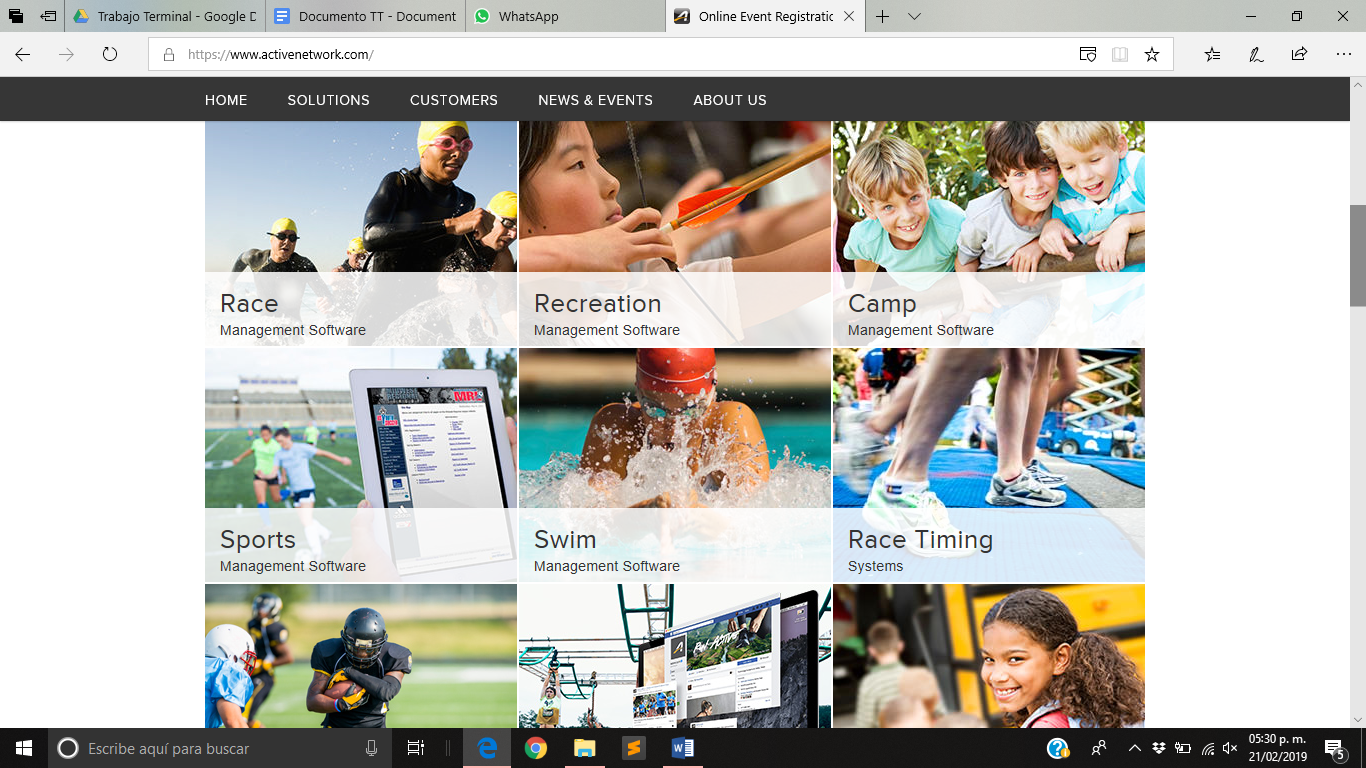
\includegraphics[width=12cm, height=6cm]{Imagenes/Aplicaciones/AN2.png}
	\caption{Eventos deportivos}
\end{figure}


\section{Aplicaciones TeamSnap Tournament}
\noindent La aplicación ofrece a los usuarios, un espacio en donde pueden registrar eventos deportivos, agendar o llevar control en el calendario de eventos, saber tablas de posiciones (estadísticas), otra característica de esta aplicación es que tiene un apartado en donde el administrador puede definir el precio de la inscripción a los eventos. \cite{team}
Características: 
\begin{itemize}
	\item Creación de eventos
	\item Dar precio para inscripción a un evento
	\item Cédula de inscripción
	\item Difusión
\end{itemize}
%=========================================================
%                                                         Imagenes
%=========================================================
\begin{figure}[hbt]
	\centering
	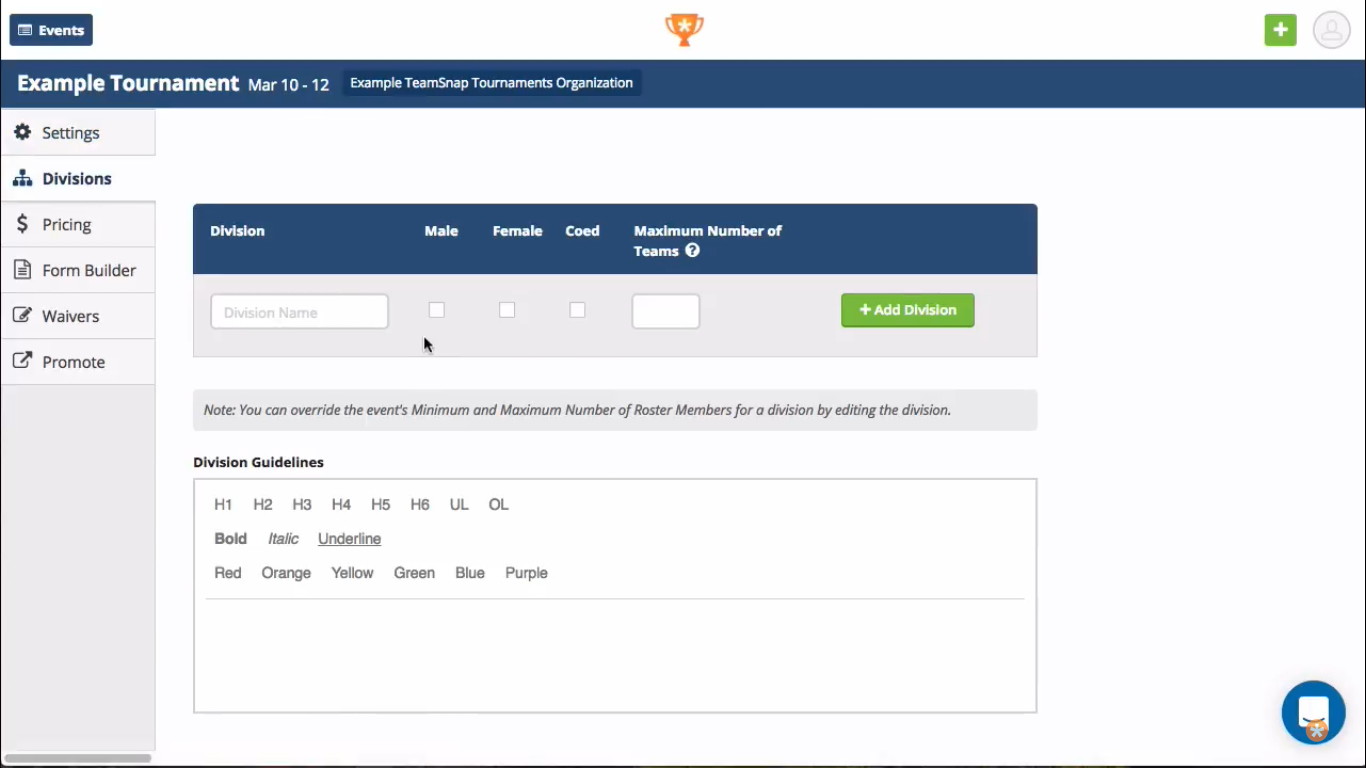
\includegraphics[width=12cm, height=6cm]{Imagenes/Aplicaciones/TsT1.png}
	\caption{Registro de competencias}
		\label{Imagen}
\end{figure}
\pagebreak
\begin{figure}[hbt]
	\centering
	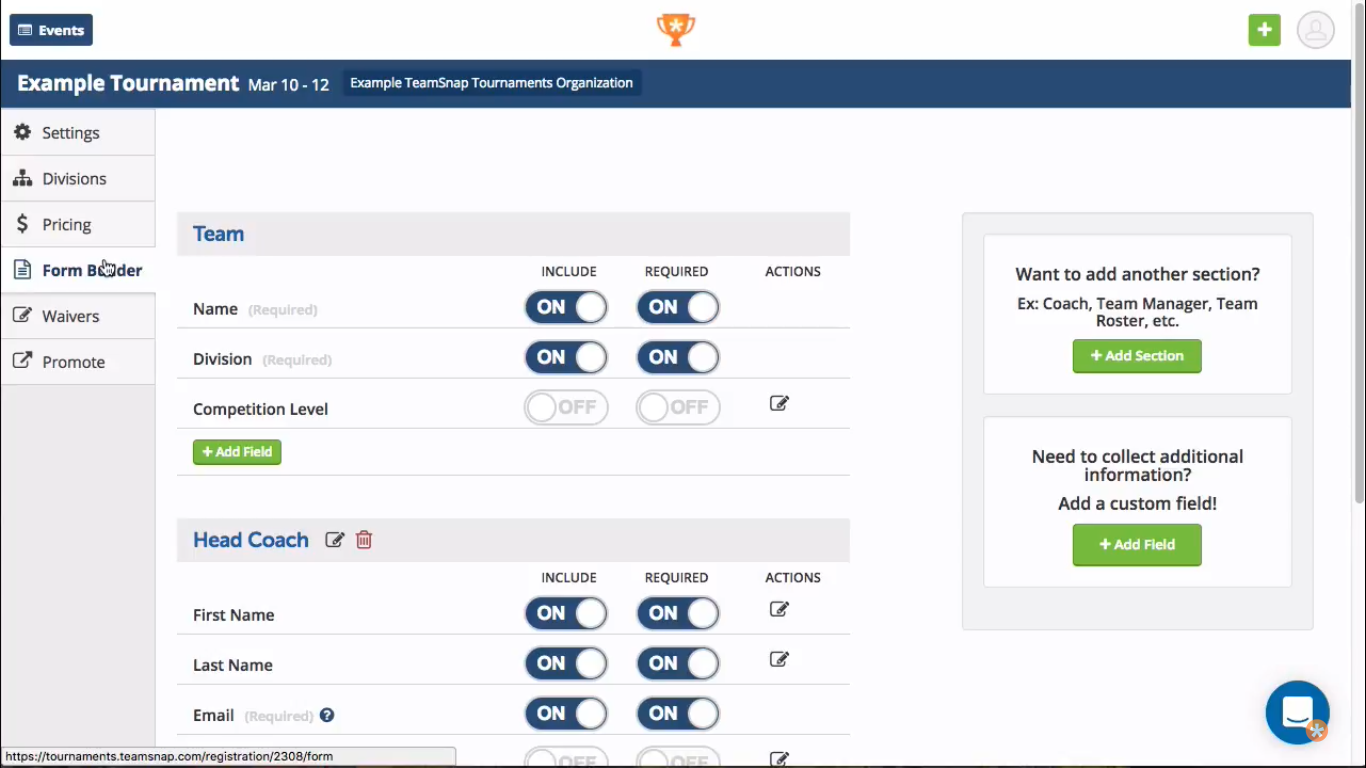
\includegraphics[width=12cm, height=6cm]{Imagenes/Aplicaciones/TsT2.png}
	\caption{Creación de cédula de inscripción}
\end{figure}
\begin{figure}[hbt]
	\centering
	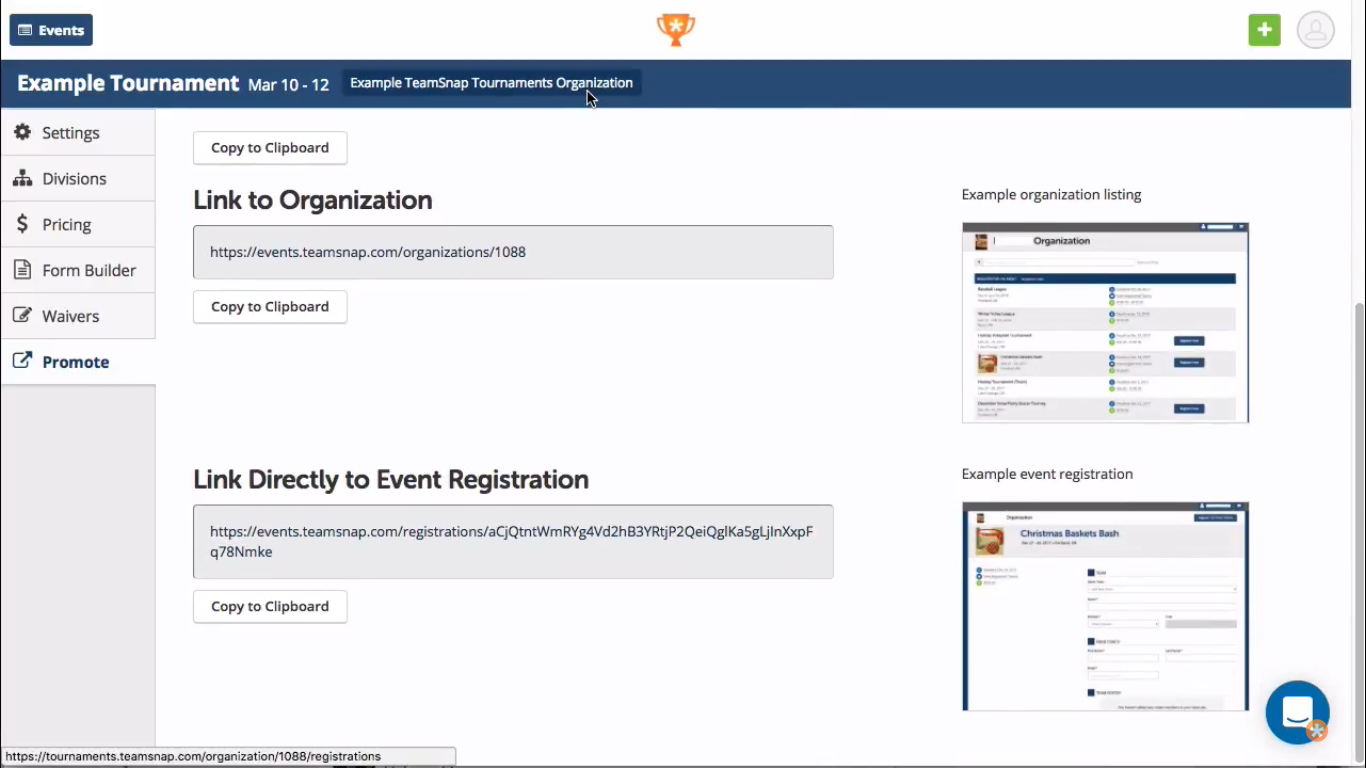
\includegraphics[width=12cm, height=6cm]{Imagenes/Aplicaciones/TsT3.png}
	\caption{Promover}
\end{figure}
\pagebreak


\section{Aplicaciones TorneoPal}
\noindent Esta aplicación, al igual que las anteriores, ofrece a los usuarios el generar un horario de actividades, generar torneos entre los equipos registrados y a su vez, en el apartado de estadísticas, ver en una tabla general el estatus de los equipos. \cite{tp}
Características: 
\begin{itemize}
	\item Creación de equipos
	\item Resultados
	\item Eliminar eventos
	\item Cambio de equipo en categorías
	\item Informe a árbitros
	\item Calendario
	
\end{itemize}
%=========================================================
%                                                         Imagenes
%=========================================================
\begin{figure}[h!]
	\centering
	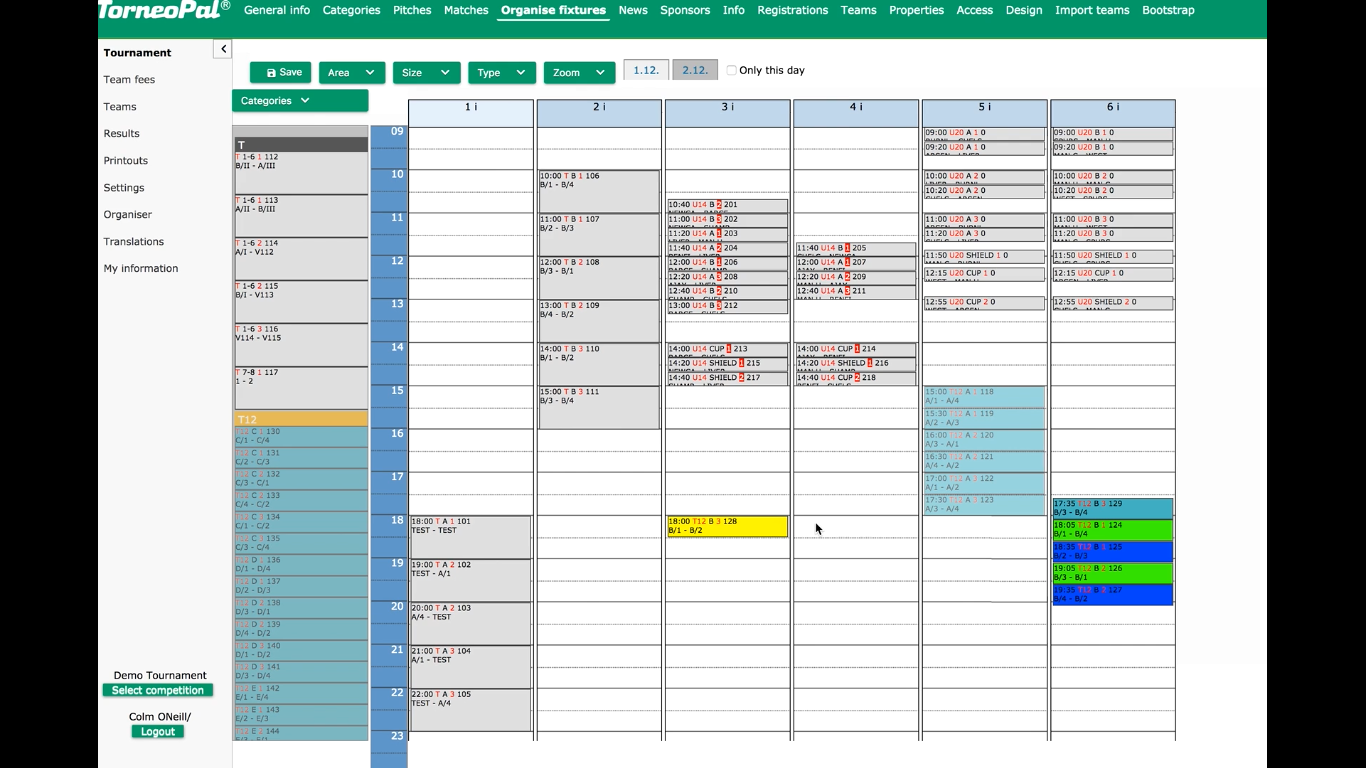
\includegraphics[width=12cm, height=6cm]{Imagenes/Aplicaciones/TP1.png}
	\caption{Calendario de eventos}
\end{figure}
\begin{figure}[h!]
	\centering
	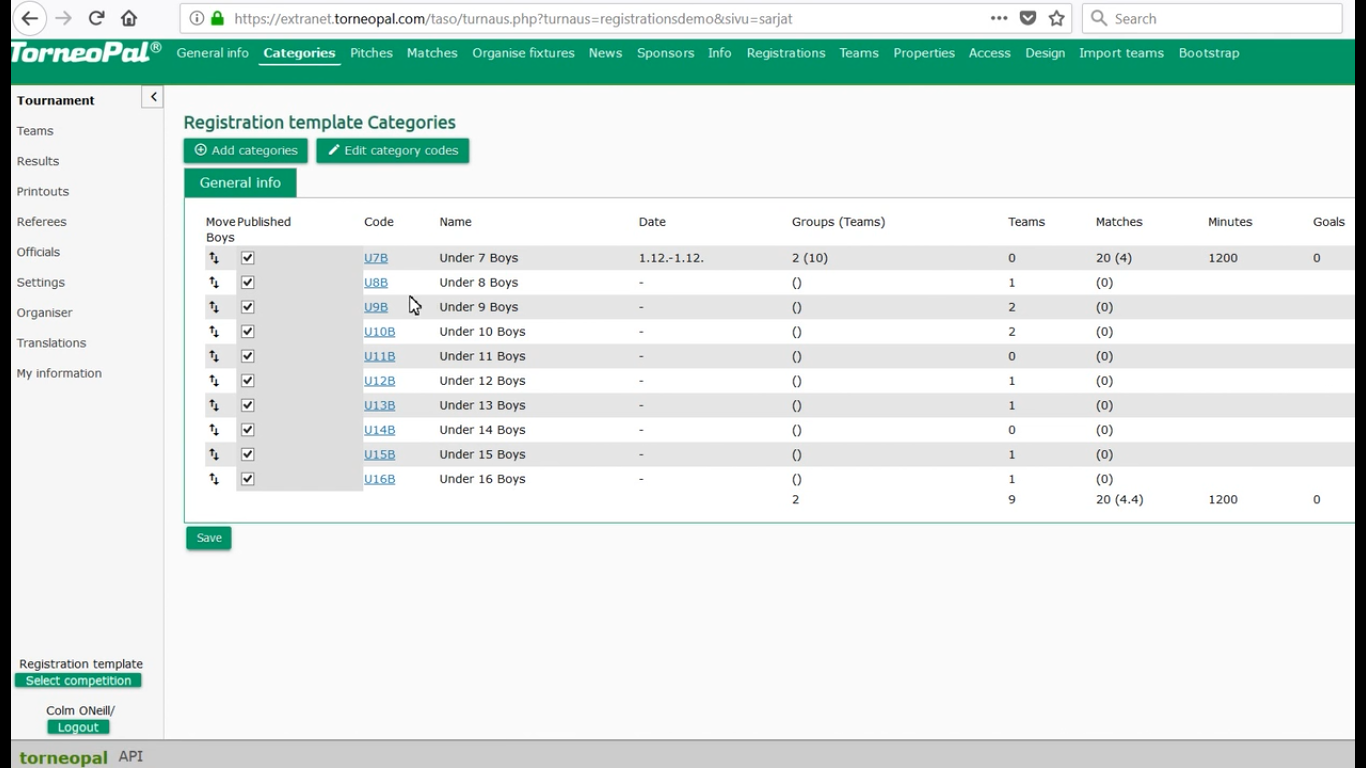
\includegraphics[width=12cm, height=6cm]{Imagenes/Aplicaciones/TP2.png}
	\caption{Registro eventos}
\end{figure}
\pagebreak

\section{Aplicaciones Instituto Nacional del deporte CHILE}
\noindent Esta aplicación está dirigida a un mercado en específico, ofreciendo dentro de esta un calendario de próximos eventos, registrarse en alguno del interés del usuario, como complemento se informa los requisitos para poder participar en los eventos y  un apartado en donde pueden dar de alta a organizaciones. No cuenta con un apartado donde muestre estadísticas. \cite{IND}
Características: 
\begin{itemize}
	\item Registro
	\item Calendario
	\item Informes
	
\end{itemize}
%=========================================================
%                                                         Imagenes
%=========================================================
\begin{figure}[hbt!]
	\centering
	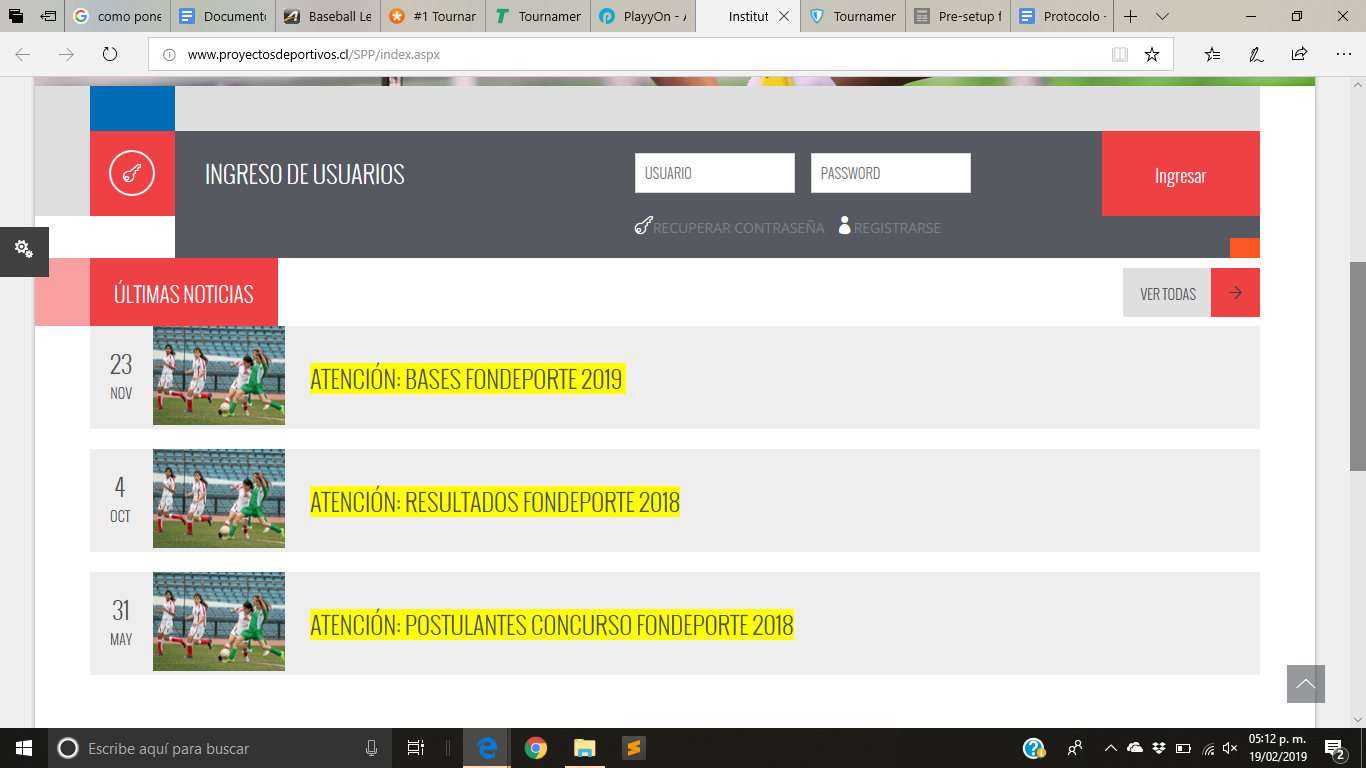
\includegraphics[width=12cm, height=6cm]{Imagenes/Aplicaciones/INDC1.png}
	\caption{Calendario de eventos}
\end{figure}
\begin{figure}[hbt!]
	\centering
	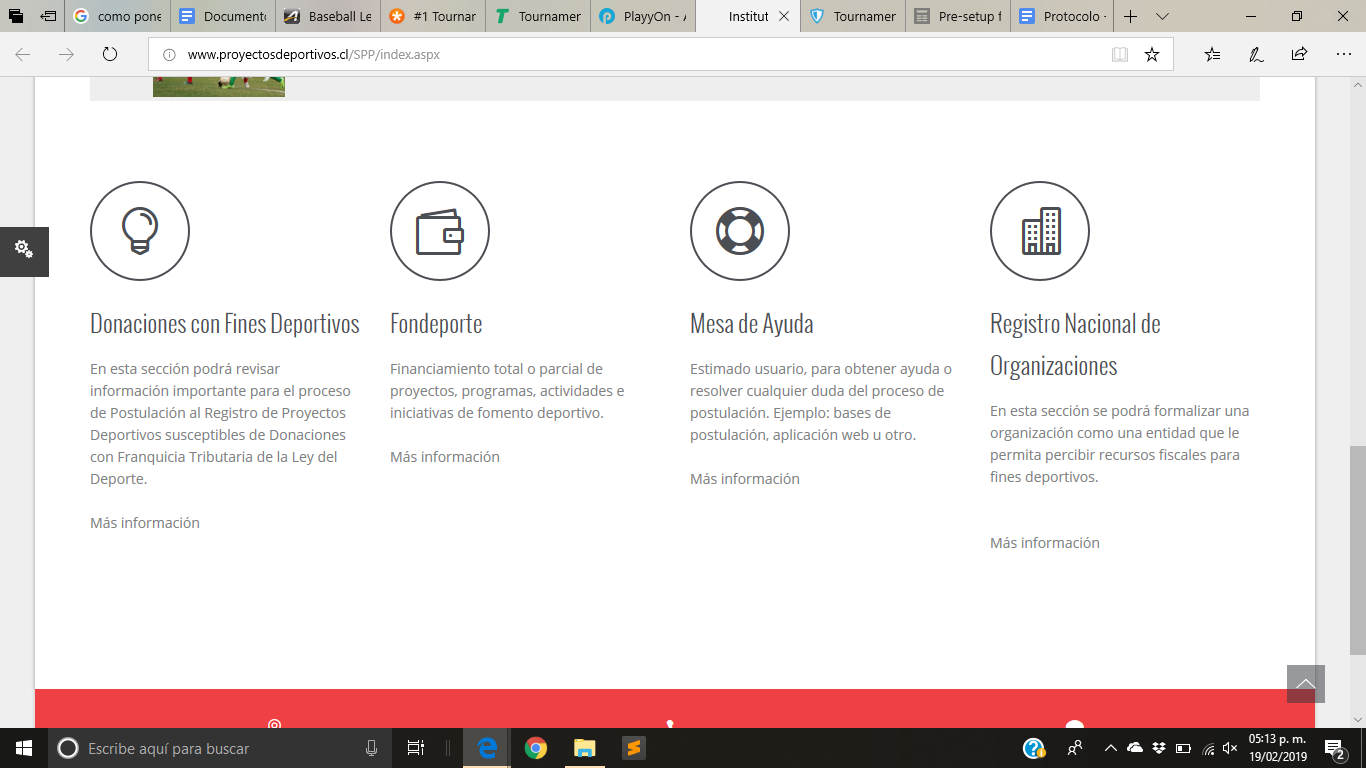
\includegraphics[width=12cm, height=6cm]{Imagenes/Aplicaciones/INDC2.png}
	\caption{Contacto}
\end{figure}
\pagebreak

\section{Prototipo para el registro a interpolitécnicos RIDESCOM}
\noindent Esta aplicación esta dirigida a la comunidad del Instituto Politécnico Nacional, especificamente en la Escuela Superior de Cómputo. La cual ofrece a la comunidad un espacio donde pueda ver el calendario de eventos próximos, resultados de la comunidad que participó, así como la posibilidad de inscribirse a un evento cuando estos esten disponibles.
Características: 
\begin{itemize}
	\item Calendario
	\item Resultados
	\item Inscripción a eventos
\end{itemize}
%=========================================================
%                                                         Imagenes
%=========================================================

\begin{figure}[hbt!]
	\centering
	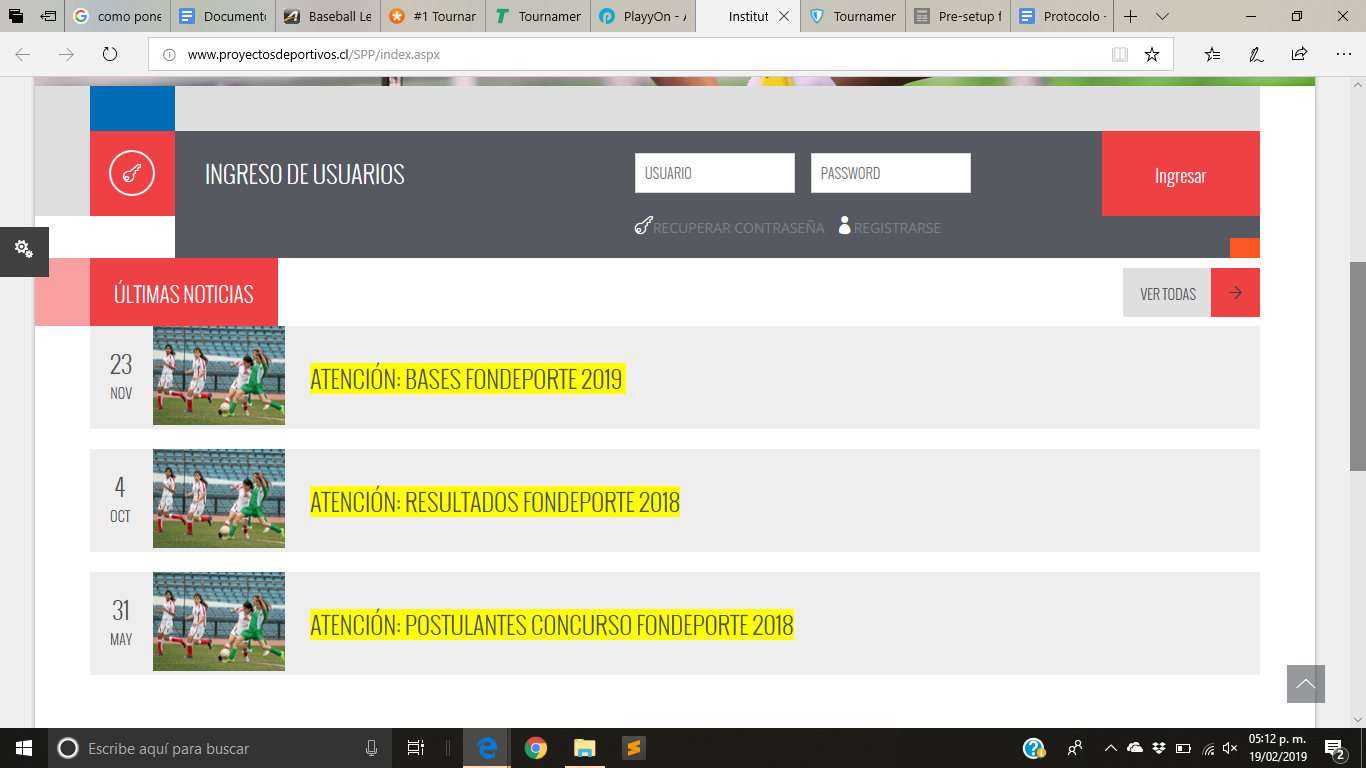
\includegraphics[width=12cm, height=6cm]{Imagenes/Aplicaciones/INDC1.png}
	\caption{Calendario de eventos}
\end{figure}
\begin{figure}[hbt!]
	\centering
	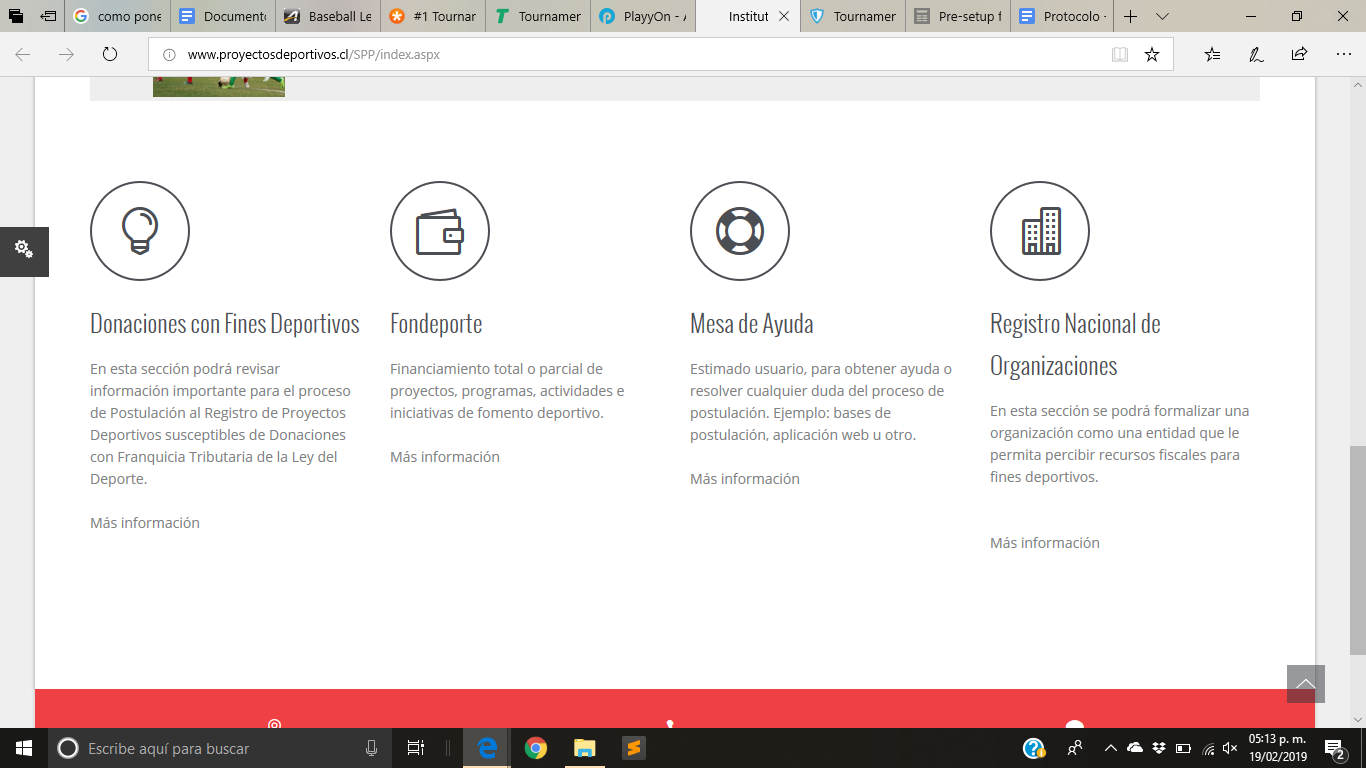
\includegraphics[width=12cm, height=6cm]{Imagenes/Aplicaciones/INDC2.png}
	\caption{Contacto}
\end{figure}